
\labday{Thursday, 18 February 2016}


\experiment{Basic Operational Amplifier Circuits - Introduction}

for the appropriate circuts we connect the 2-Output SC Power SUpply in Series to get -15V and +15V; the middle Point(Point of connection between + of one and - of the oterh is connected to GND to have GND as reference).





\experiment{The Voltage Follower}
\begin{figure}[H] % Example of including images
\begin{center}
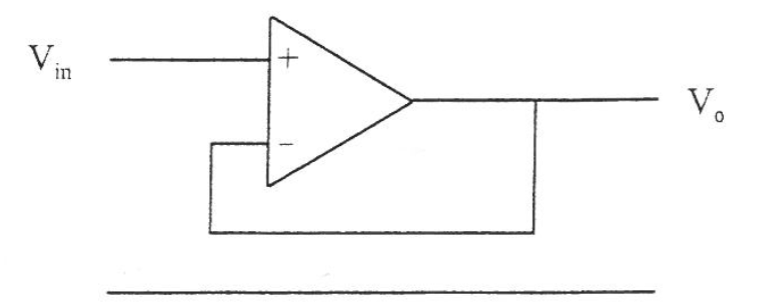
\includegraphics[width=1\linewidth]{LabTwo/a}
\end{center}
\caption{Circuit A, the voltage follower}
\label{fig:2_voltage}
\end{figure}

\subexperiment{Procedure}
\begin{enumerate}
	
\item Connect up the circuit of the voltage follower shown in Circuit A below using a $\pm$ 15 V
supply for the Op-amp.
\item  Connect the input to ground, 0 Volts, and measure the dc output voltage using the multimeter. This is the output off-set voltage.
\item  Apply a suitable dc voltage to the input, measure it and the dc output voltage and calculate
the dc gain.
\item  Apply a suitable ac voltage to the input and observe the output voltage on the oscilloscope.
Measure the ac input voltage and the ac output voltage and calculate the ac gain.
\end{enumerate}

\subexperiment{Results}
%2) applied 0 Volts -> output offset voltage: 2.5mV
%3) measured: 5.03V at 5.02V applied -> Gain is 0.01V
%4) AC Voltage RMS set to 0.302V -> Peak Value 2V (see pic) -> output ac value is as well 2V peak to peak (DC offset at bottom!) -> Gain is 2


After connecting the 2-Output DC-Power Supply to a configuration that allows +15V and -15V Output as well as Ground (connecting the two Power Outputs in series, Ground reference taken from the middle of the connection) and connecting the circuit, the power supply is switched on.
Now the Output Voltage is measured with a multimeter, which gives a value of \textbf{2.5mV}, which corresponds to the output offset voltage.
\newline
Now the input voltage is replaced with a 5.02V DC input provided by another DC Power Supply.
\newline
Measuring the Output Voltage again with the Voltmeter, gives a value of \textbf{5.03V}, which results in a gain of \textbf{0.1V}.


Now the DC input is replaced with an AC input, set to 0.302V RMS, and the oscilloscope is connected. Measuring the Peak-to-Peak value of the curve (see image \todo{add image here and calculate proper gains!} ) gives a peak value of about 2V (the bottom is a bit more, because of the DC offset!), therefore the AC Gain is 2.




\experiment{The Non-inverting Amplifier}

\begin{figure}[H] % Example of including images
\begin{center}
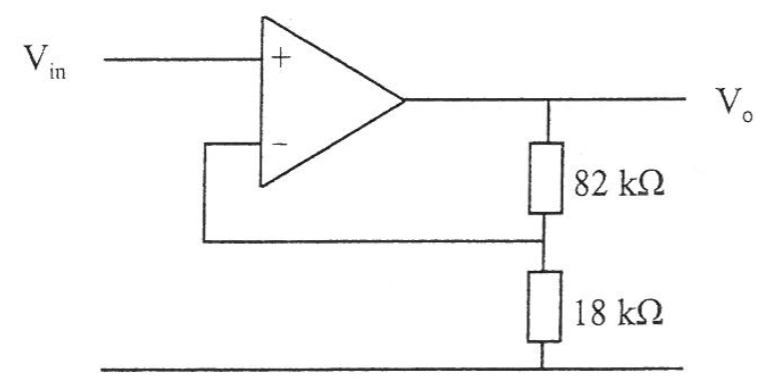
\includegraphics[width=1\linewidth]{LabTwo/b}
\end{center}
\caption{Circuit B, the non-inverting amplifier}
\label{fig:2_noninv}
\end{figure}

\subexperiment{Procedure}

\begin{enumerate}
	\item Connect up the circuit of the non-inverting amplifier shown in Circuit B by modifying the
above circuit A.

	\item Repeat the steps 2, 3, and 4 of Procedure A above for this circuit.

	\item Apply a square wave input to V$_{in}$ and observe the output voltage on the oscilloscope.
Measure the slew rate of the amplifier output.
\end{enumerate}

\subexperiment{Results}
%modifying Circuit of A -> R_82 is R = 81.85 kOhm; R2 = 17.52kOhm 
%
%2) apply 0 Volta -> output ofset voltage: 24.7 mV
%3) DC VOltage input 0.992V; measured: 5.51V
%4) AC voltage input: peak to peak: 1V; -> (picture scope 17) peak to peak 5.6 Volt
%
%Chip burned twice -> turned off opa amp power supply before turning off the input power
%5) slew rate -> picture 19 or something; peak to peak voltage is 6.1; rise time 5.752; slew rate 6.1V / (1.5us * 5 us) = 0.813 us/V

Now the circuit from the previous experiment is modified by adding two Resistors R$_{82}$ and R$_{18}$. Verifying the resistors with the resistor measurement device gives R$_{82}$ = 81.85 k$\Omega$ and R$_{18}$ = 17.52 k$\Omega$.

Again, 0 Volts are applied and the output is measured with a multimeter, which gives 24.7 mV, the output offset voltage.

The 0V input is now replaced by a 0.992V DC input, and the output is measured again: 5.51V. \todo{calculate gain here}.
\newline
After measuring, the OpAmp started to smoke and we shut off all power supplies. We suspect a short circuit somewhere in the wiring, but could not see any problem. Therefore we dismantled the whole circuit \& power supply wiring and wired it again.
Since we had the measurement for the DC input already and were short on time, we decided to continue with the AC measurement.

After reconnecting and checking the circuit again, we connect the AC input with a peak-to-peak voltage of 1V \todo{add picture here, should be image 17 or something}. Measuring the output with the oscilloscope gives us a peak-to-peak voltage of 5.6V. After the measurement we again experienced the issue described above. Even now we could not find any short-circuit in the wiring.

 A small investigation led us to the conclusion, that we switched off the OpAmp Power Supply before turning off the OpAmp Input, which is most likely the causing issue for the disintegration of the OpAmps.
 
 Re-wiring and measuring again, gives us now a value of 6.1V Peak to Peak (with 1V peak-to-peak input) when AC input is applied. \todo{add image here, pic 19}
 Now we could measure the slew rate of 0.813 uS/V, with a rise time of 5.752s.
 
 
 


\experiment{The Current to Voltage Amplifier}
\begin{figure}[H] % Example of including images
\begin{center}
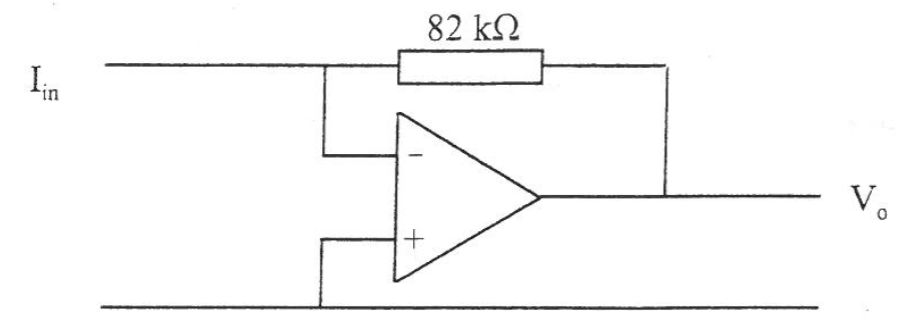
\includegraphics[width=1\linewidth]{LabTwo/c}
\end{center}
\caption{Circuit C, the current to voltage amplifier}
\label{fig:2_currentToVoltage}
\end{figure}


\subexperiment{Procedure}
\begin{enumerate}
	\item Connect up the circuit of the current to voltage amplifier shown in Circuit C below again using a $\pm$ 15 supply for the Op-amp.

	\item Connect the input to ground, 0 Volts, and measure the dc output voltage using the multimeter. This is the output off-set voltage.

	\item To measure the input current to output voltage ratios, for do and for ac, for this circuit
requires do and ac input currents. These can be obtained from appropriate voltage sources
via suitable values of resistor. For the do and ac measurements decide on a value of current
that will give you a convenient output voltage and choose suitable source voltages and
resistor values to give these. For each apply the current to the input and measure it and the
output voltage. Calculate the dc and the ac transfer impedances.

\end{enumerate}

\subexperiment{Results}
%Using again 82kOhm from before and a 10kOhm resistor (because it was available) -> this results in Vout of 8.2, with a current of 1mA -> nope, using 18kOhm to get 4.55V in the end as output;
%at first we got with input of 0V an output of about 13V; -> 71.5mV in the ned -> because cable was wrong connected;
%2) input DC 0.991V -> output oltage 4.41V
%3) AC input: 1V peak to peak; putput: 4.7V(scope 21)
%
After connecting and checking the wiring and applying 0V to the OpAmp input we measured a output offset voltage of 71.5mV.

Calculating an appropriate resistor value \todo{include here how done} gave us a resistor value of 18 k$\Omega$ to have an voltage output of about 5V.
Using the resistors from the experiment before and measuring the output by applying a DC input voltage of 0.991V, we obtained a V$_Out$ of 4.55V, which is quite close to the calculated value.

Again, this measurement was done using a AC power input of 1V peak-to-peak \todo{add image 21 here} resulting in a voltage output of 4.7V.
\todo{calculatee the DC and AC transfer impedances}




\experiment{The Inverting Amplifier}

\begin{figure}[H] % Example of including images
\begin{center}
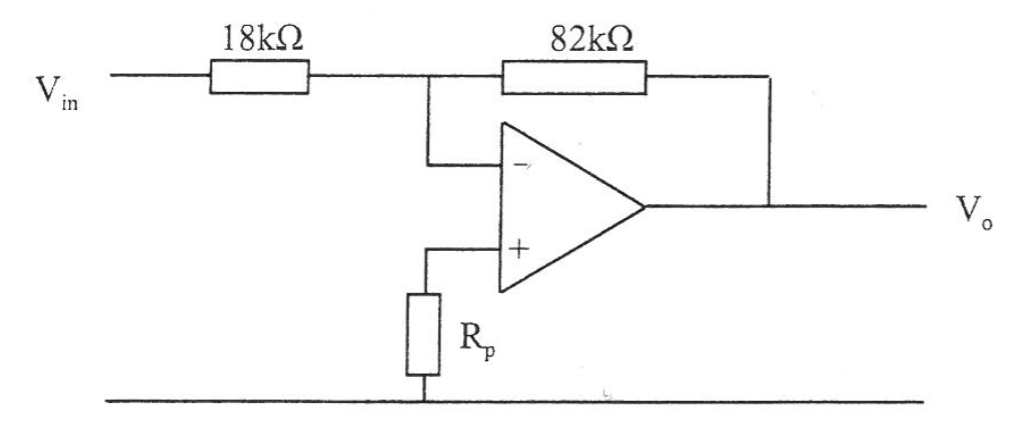
\includegraphics[width=1\linewidth]{LabTwo/d}
\end{center}
\caption{Circuit D, the inverting amplifier}
\label{fig:2_inverting}
\end{figure}

\subexperiment{Procedure}
\begin{enumerate}
	\item Connect up the circuit of the inverting amplifier shown in Circuit D by modifying the
above circuit C. This involves the calculation of a suitable value for the resistor Rp.
\item Repeat the steps 2, 3, and 4 of Procedure A above for this circuit.

\end{enumerate}
\subexperiment{Results}
%R_p should be 14.76kOhm (see lecture; because of imperfections) -> using 14.962kOhm
%2) 53.9mV dc offset
%3) DC input votlage: 0.991V (gain should be -4.555) DC output voltage: -4.42V
%4) AC peak to peak: 1V (pic 22)

Calculating an appropriate R$_P$ is done as stated in the lecture on OpAmps, and results in a value of R$_P$ = 14.76 k$\Omega$. After selecting a resistor with the closest value (14.962 k$\Omega$, verified with the resistance measurement device), we again applied 0V to the input.

This results in a DC offset voltage of 53.9mV.

Applying a DC input voltage of 0.991V, we measure -4.42V at the OpAmp output, which corresponds to the theoretical calculated gain value of -4.55.

Applying a AC input voltage of 1V peak-to-peak we obtain \todo{get the image here!}





\experiment{The Summing Amplifier}
\begin{figure}[H] % Example of including images
\begin{center}
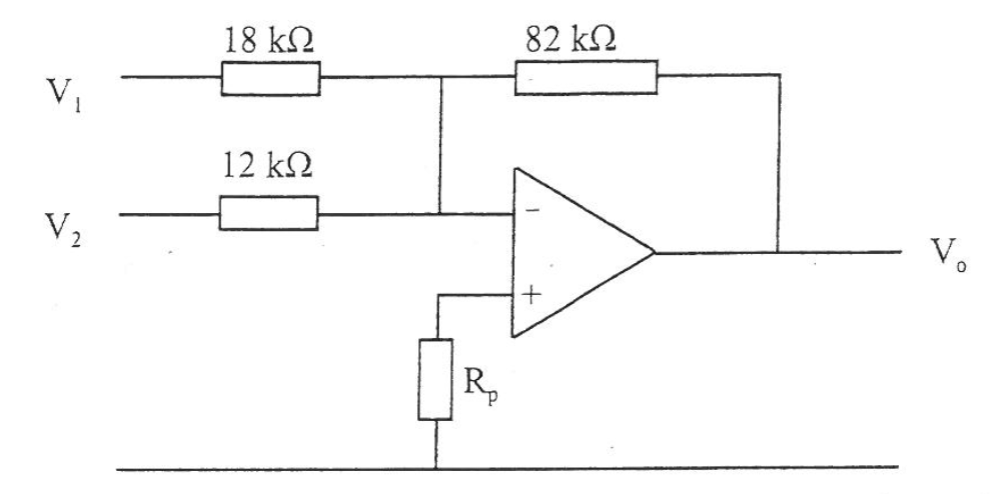
\includegraphics[width=1\linewidth]{LabTwo/e}
\end{center}
\caption{Circuit E, the summing amplifier}
\label{fig:2_summing}
\end{figure}

\subexperiment{Procedure}
\begin{enumerate}
	\item Connect up the circuit of the inverting amplifier shown in Circuit E by modifying the above
circuit D. This involves the recalculation of a suitable value for the resistor R1,

	\item Connect both of the inputs to ground, 0 Volts, and measure the dc output voltage using the
multi-meter. This is the output off-set voltage.


	\item Apply two suitable dc voltages one to each of the inputs, measure them and the dc output
voltage and calculate the relationship between the input voltages and the output voltage.


	\item Apply a suitable ac voltage to one input and say a square wave of a to the other input,
inspect these and the output voltage using the oscilloscope and print out the appropriate
screens. Account for the output voltage waveform in terms of the input voltages and the
relationship between the inputs and the output. Vary the frequency of one of the inputs and
inspect the results.

\end{enumerate}
\subexperiment{Results}
%Recalculation of Rp: 6.8 -> using 6.778kOhm
%using 11.957kOhm for R_2
%
%Applying 0V to both inputs: 119.6mV
%2) now apply  0.488V to both inputs -> V 5.39V
%theoretical : -5.55
%3) AC voltage: 0.6V peak to peak
%-> not using AC AC , but DC of 0.488V and AC of 0.5V peak to peak ; AC as swaure wave
%-> very noisy with small values
%using now AC Voltage (sine wave) -> recalculated (picture 23) -> varying the AC input makes the picture clearer =P
%

After modifying the circuit to match the wanted Circuit given in FIgure \todo{ref einfügen}, recalculation of the R$_P$ value gives a resistance of 6.9 k$\Omega$. We again use the closest resistor we can find (6.778 k$\Omega$, verified with the resistance measurement device).
For R$_2$ a resistor with the value of 11.957 k$\Omega$ is used.

Connecting both inputs to 0V results in an output of 119.6mV.

Applying 0.448V to both inputs, results in an output of 5.39V, which matches the theoretical calculated value of 5.55V. \todo{calculate relationship bla}

Now, other than stated in the procedure, we were advised to use one AC and one DC input instead of a square wave input.
We now apply a DC input with 0.448V and a AC (sine wave) with a peak value of 0.5V.
Picture \todo{insert image 23}




\experiment{The Differential Amplifier}
\begin{figure}[H] % Example of including images
\begin{center}
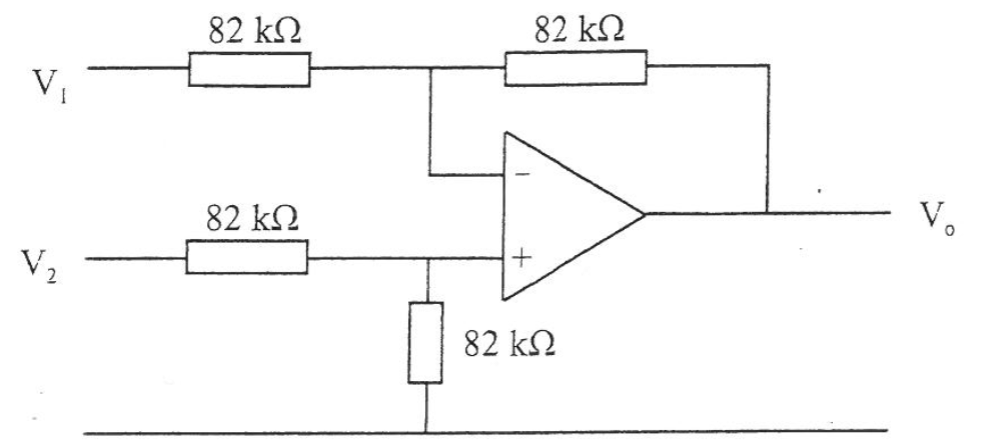
\includegraphics[width=1\linewidth]{LabTwo/f}
\end{center}
\caption{Circuit F, the differential amplifier}
\label{fig:2_diffAmp}
\end{figure}

\subexperiment{Procedure}
\begin{enumerate}
	\item  Connect up the circuit of the differential amplifier shown in Circuit F below using a $\pm$ 15
supply for the op-amp and noting that all the resistors are identical in value.
\item  Connect both of the inputs to ground, 0 Volts, and measure the dc output voltage using the
multi-meter. This is the output off-set voltage.

\item  Connect the two inputs together and apply a large voltage (say 10 Volts) to them. Measure
this input voltage and the output voltage and calculate the common mode gain, hopefully
less than unity. You can consider subtracting the output off-set voltage from the common
mode output voltage before calculating the common mode gain.

\item Apply two very different values of dc voltage one to each of the inputs, measure them and
the dc output voltage and calculate the relationship between the input voltages and the
output voltage.

\item  Repeat 4 with the two input voltages exchanged.

\item  Apply two very similar but large values (say around 10 Volts) of dc voltage one to each of
the inputs, measure them and the dc output voltage and calculate the relationship between
the input voltages and the output voltage.

\item  Repeat 6 with the two input voltages exchanged.
\end{enumerate}

\subexperiment{Results}
%2) offset -> 20.0mV
%3) setting INput voltage to 9.79V; measured output: 20.3mV
%V2 -> 4.98V
%V1 -> 7.19V
%-> Vout 2.188V
%now switch the V2 and V1
%-> Vout 2.242V
%5) V1 9.99V as input ; V2 = 10.56V -> output 0.607V
%6) switch them now -> Vout ->-0.544V

We again modified the circuit to match the one given in figure \todo{insert ref}
\begin{enumerate}
	\item Applying 0V input and measuring the output, results in a dc offset voltage of 20.0mV
	\item After setting the input voltages to 9.79V (connected together), we obtain a measured output voltage of 20.3mV, which matches our expectations. 
		Now we modify the input voltages, so that V$_1$ = 7.19V and V$_2$ = 4.98V. This gives us an output of 2.188V. 
		Switching these inputs results again in an voltage output of 2.242V. \todo{alc relationship between the in and out}
	\item Now we set V$_1$ = 9.99V and V$_2$ = 10.56V. This results in a voltage output measurement of 0.607V. Switching the inputs again gives a $V_{out}$ = 0.544V
\end{enumerate}



\experiment{The Schmitt Trigger Comparator}

\begin{figure}[H] % Example of including images
\begin{center}
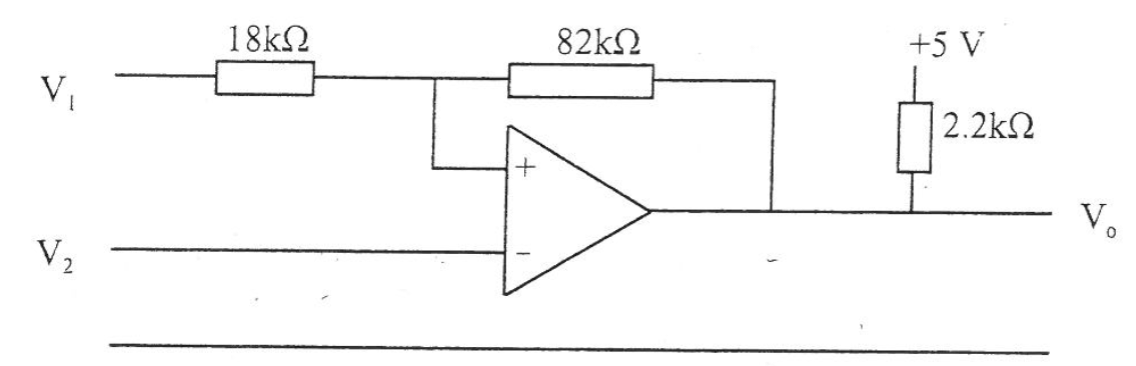
\includegraphics[width=1\linewidth]{LabTwo/g}
\end{center}
\caption{Circuit G, the Schmitt Trigger Comparator}
\label{fig:2_voltage}
\end{figure}


\subexperiment{Procedure}
\begin{enumerate}
	\item Connect up the circuit of the Schmitt Trigger Comparator circuit shown in Circuit G below using a $\pm$ 15 Volt supply for the LM 311 comparator.
\item Connect input V$_2$ to Ground and apply a variable DC voltage at V$_1$. Starting with V$_1$ negative and the output at 0 Volts increase the voltage on V$_1$ and note the value of V$_I$ at which the
output switches to +5 Volts. Then decrease the voltage on V$_I$ until the output again switches
to O Volts and note the voltage on V$_I$ at this point.

\item Apply a saw tooth waveform to V$_2$ at a frequency of 10 kHz and observe the output
waveform and the sawtooth input waveform on the oscilloscope. Vary the dc voltage on V$_I$
and observe the variation in the width of the pulses at the output. This is known as pulse
width modulation.

\item Using the oscilloscope measure the slew rate of the comparator and compare it with that of
the op-amp.
\end{enumerate}

\subexperiment{Results}

After rewiring and connecting the power supply we were advised to skip number 2 of the procedure.
For the circuit the following resistor values were used (verified with the resistor measurement device): R$_{2.2}$ = 2.1959 k$\Omega$, R$_{82}$ = 81.77 k$\Omega$ and R$_{18}$ = 17.991 k$\Omega$.


Now we applied a waveform at a frequency of 10 kHz to V$_2$ and observed the waveform on the oscilloscope (see figures \todo{insert images}).
Measuring the slew rate with the oscilloscope we obtained a slew rate of 150ns (see images 27 and 28 \todo{insert images}.
%
%R_2.2 ->  2.1959kOhm
%82 -> 81.77
%18 -> 17.991
%
%second part:
%
%
%slew rate -> 150ns
%see pic 27
%
%see pic 28 (use 10\% and 90\% for the measurements)
%12V -> per microseconds

